% Simple poster (portrait)
% Author: Sofia Jijon (https://sjijon.github.io)
% Last Update: Sept 9, 2021
% Latest Version: https://github.com/sjijon/TeX-templates/tree/main/Tikzposter%20posters/Simple%20poster

\documentclass[a0paper,portrait,margin=0pt, colspace=24pt,subcolspace=0pt,blockverticalspace=36pt,innermargin=50pt]{tikzposter}
\usepackage[utf8]{inputenc}


\usepackage[T1]{fontenc}
\usepackage[square,numbers]{natbib} 	% Bibliography manager
\usepackage{amsmath,amssymb}
\usepackage{lipsum}  				    % Random Text
\usepackage[colalign]{aligncolsatbottom}  %To align columns at bottom (!! please run 2 times)

%..............................................................................................................................................................................................
% Display
\tikzposterlatexaffectionproofoff 			
\usetikzlibrary{shapes.geometric,arrows.meta,positioning}  %Tikz Libraries

% Fonts
\usepackage{helvet}					% Sans-Serif
\renewcommand{\familydefault}{\sfdefault}	%

% Colors
	\definecolor{MyOrange}{rgb}{0.8, 0.33, 0}
	\definecolor{MyBrown}{rgb}{0.28, 0.20, 0.20}
	\definecolor{MyGreen}{rgb}{0.33, 0.42, 0.18}

% Theme
\usetheme{Default}
\definecolorstyle{MyStyle2016}{
	\definecolor{ColorOne}{named}{MyBrown} 
	\definecolor{ColorTwo}{named}{MyOrange}
	\definecolor{ColorThree}{named}{MyGreen}
}{
    % Title Colors
    \colorlet{titlebgcolor}{ColorOne}
    \colorlet{titlefgcolor}{white}
    % Background Colors
    \colorlet{backgroundcolor}{ColorOne!15}
    \colorlet{framecolor}{ColorOne}
    % Block Colors
    \colorlet{blocktitlebgcolor}{white}
    \colorlet{blocktitlefgcolor}{ColorTwo}
    \colorlet{blockbodybgcolor}{white}
    \colorlet{blockbodyfgcolor}{black}
    % Innerblock Colors
    \colorlet{innerblocktitlebgcolor}{ColorOne!15}
    \colorlet{innerblocktitlefgcolor}{black}
    \colorlet{innerblockbodybgcolor}{ColorOne!15}
    \colorlet{innerblockbodyfgcolor}{black}
    % Note colors
    \colorlet{notebgcolor}{ColorTwo!20}
    \colorlet{notefgcolor}{ColorTwo}
    \colorlet{notefrcolor}{ColorTwo}
 }

% Color style
\usecolorstyle{MyStyle2016}
%..............................................................................................................................................................................................
\title{KARŞILAŞTIRMALI ÖRNEKLERLE ZAMAN SERİSİ KULLANIMLARI     }

\author{RUMEYSA NUR BALABEY\textsuperscript{1}, \underline{ALPER SİNAN ÇALIK}\textsuperscript{1,2}, DENİZ BALCI\textsuperscript{2}}

\institute{	\textbf{https://github.com/SirmaXX/veri$\_$gorsellestirme$\_$odevi$\# $veri$\_$gorsellestirme$\_$odevi}}

%..............................................................................................................................................................................................
\begin{document}
%
%
%	HEAD
%
%....................................................................................
%
%	Title
%
\maketitle[width=0.96\linewidth,titletoblockverticalspace=36pt,linewidth=0,roundedcorners=10]
%..............................................................................................................................................................................................
%
%	Block
%
\block[titleleft,roundedcorners=16]{ÖZET}{
	
	 }

%..............................................................................................................................................................................................
%
%	LEFT COLUMN
%
\begin{columns}
\column{0.50}
%....................................................................................

\block[titleleft,roundedcorners=16]{Yıllara göre Dolar Türk Lirası ve Ereğli Demir çelik Fiyat Değişimi}{
	\raggedleft

		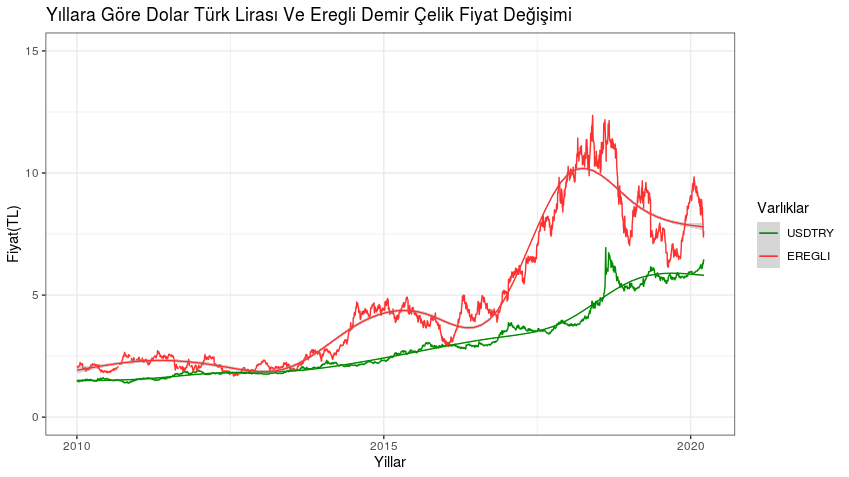
\includegraphics[width=1\linewidth]{A very simple poster/Figures/1.png}

}
%....................................................................................
%
%	Block
%
\block[titleleft,roundedcorners=16]{Model Block}{
		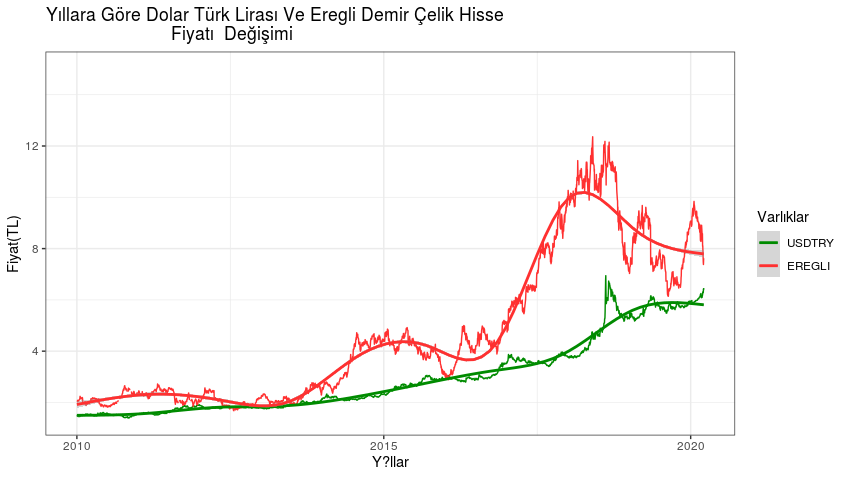
\includegraphics[width=1\linewidth]{A very simple poster/Figures/2.png}
	 }

%..............................................................................................................................................................................................

% 	RIGHT COLUMN
%
\column{0.50}
%%....................................................................................
%
%	Block
%
\block[titleleft,roundedcorners=16]{Another block}{
	\raggedleft

		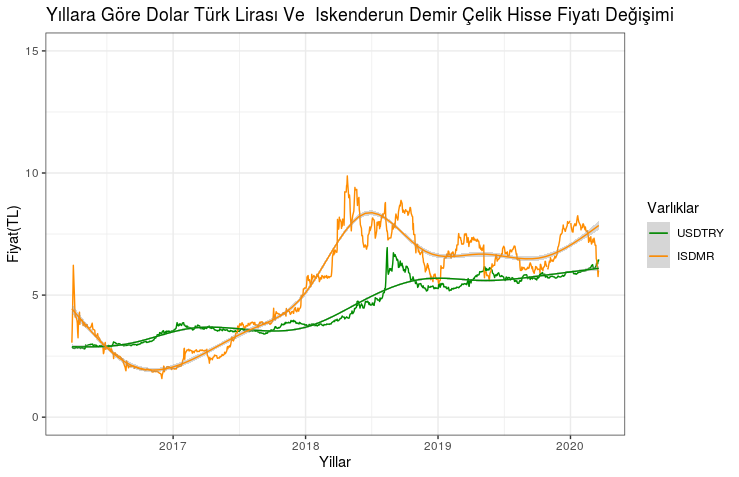
\includegraphics[width=1\linewidth]{A very simple poster/Figures/3.png}
	
	}
%....................................................................................
%
%	Block
%
%
%	Block
%
\block[titleleft,roundedcorners=16]{Another block}{
	\raggedleft

		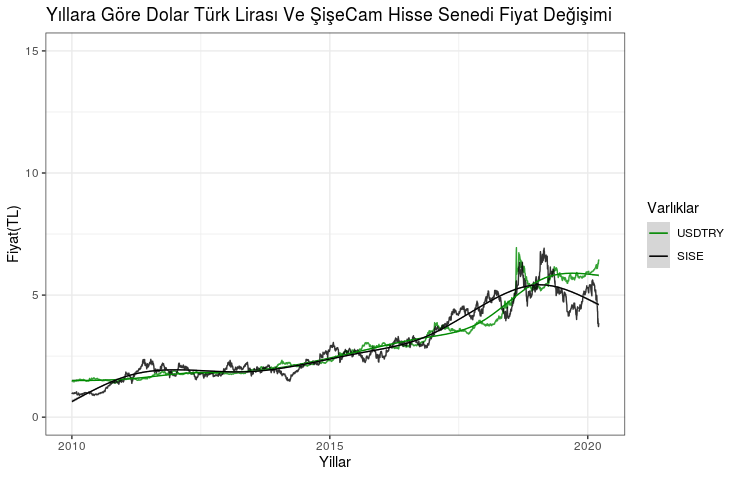
\includegraphics[width=1\linewidth]{A very simple poster/Figures/4.png}
	
	}
%....................................................................................
%
%	Block
%

\end{columns} 
%..............................................................................................................................................................................................
%
%	FOOT
%
%....................................................................................
%
%	References
%
\block[titleleft,roundedcorners=16]{Sonuç}{
	\raggedright

 }
 
 
\block[titleleft,roundedcorners=16]{}{
\small
\begin{minipage}{0.73\linewidth}
	\nocite{*}
	\bibliographystyle{unsrtnat}
	\bibliography{BibPoster}
 \end{minipage}
%....................................................................................
%
%	Logos
%
\begin{minipage}{0.2\linewidth}
\centering
	
\includegraphics[height=5cm]{A very simple poster/Figures/index.png}
\end{minipage}
}
%....................................................................................
%
%	My info
%

\end{document}